\chapter{Análisis transitorio}

\section{Enunciado}
En el circuito de la figura, el interruptor ha estado abierto durante un tiempo
prolongado, y en el instante $t = 0$ se cierra. Se debe determinar el valor de las tensiones y corrientes del circuito en $t = 0^+$.

\begin{minipage}{0.5\linewidth}
  \center{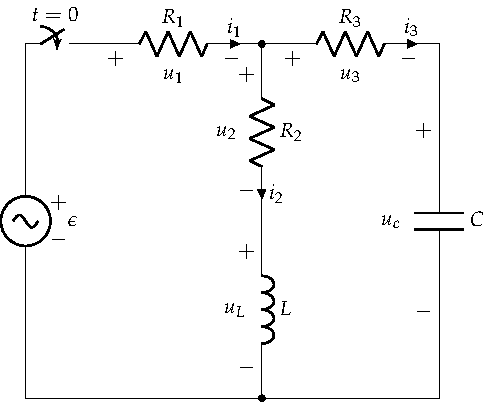
\includegraphics{figuras/BT4_CondicionesIniciales_bobcon.pdf}}
\end{minipage}
\begin{minipage}{0.5\linewidth}
  \center{Datos:}
  \begin{align*}
    R_1 &= 3\,\unit{\ohm}\\
    R_2 &= 5\,\unit{\ohm}\\
    R_3 &= 2\,\unit{\ohm}\\
    L &= 0.2\,\unit{\henry}\\
    C &= 0.5\,\unit{\milli\farad}\\
    \epsilon(t) &= 20\cos(t)\,\unit{\volt}
  \end{align*}
\end{minipage}

\subsection*{Solución}

En $t < 0$, dado que el interruptor ha estado abierto, la bobina y el condensador están descargados. Por tanto, $i_2(0^-) = \qty{0}{\ampere}$ y $u_C(0^-) = \qty{0}{\volt}$.

\smallskip
\begin{minipage}{0.5\linewidth}
En $t > 0$, al cerrarse el interruptor, la fuente de tensión alimenta al circuito. En el instante de cierre, $\epsilon(0^+) = \qty{20}{\volt}$. Por otra parte, aplicando el principio de continuidad en la bobina y el condensador, tenemos:
\begin{align*}
  i_2(0^+) &= i_2(0^-) = \qty{0}{\ampere}\\
  u_C(0^+) &= u_C(0^-) = \qty{0}{\volt}
\end{align*}
Estos resultados implican que, en ese instante, la bobina se comporta como un circuito abierto y el condensador como un cortocircuito. 
\end{minipage}
\begin{minipage}{0.5\linewidth}
  \center{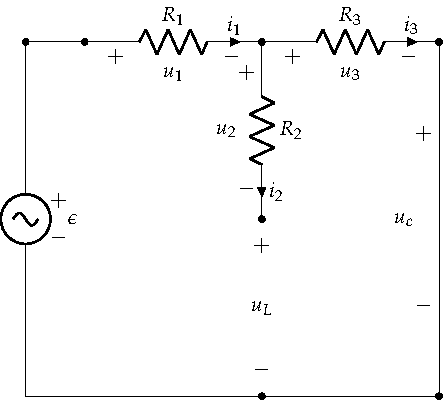
\includegraphics[scale=0.95]{figuras/BT4_CondicionesIniciales_bobcon0+.pdf}}
\end{minipage}
\smallskip

En estas condiciones calculamos el resto de variables en $t = 0^+$:
\begin{align*}
  i_1(0^+) = i_3(0^+) &= \frac{\epsilon(0^+)}{R_1 + R_3} = \qty{4}{\ampere}\\
  u_1(0^+) &= R_1 \cdot i_1(0^+) = \qty{12}{\volt}\\
  u_2(0^+) &= R_2 \cdot i_2(0^+) = \qty{0}{\volt}\\
  u_3(0^+) &= R_3 \cdot i_3(0^+) = \qty{8}{\volt}\\
  u_L(0^+) &= u_3(0^+) = \qty{8}{\volt}
\end{align*}

\section{Enunciado}
El interruptor de la figura lleva cerrado un tiempo que se puede
  considerar infinito. En el instante $t=0$, se abre, permaneciendo en
  esta posición definitivamente. Calcular la expresión de la
  intensidad $i(t)$ desde $t=0$ en adelante.  
  
  Datos:\;
  $E = \qty{1}{\volt}$;\; $R_1 = \qty{1}{\ohm}$;\;
  $R_2 = R_3 = \qty{2}{\ohm}$;\; $C = \qty{4}{\milli\farad}$

\begin{center}
  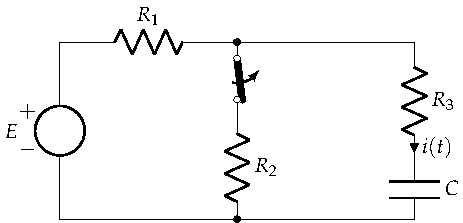
\includegraphics{figuras/BT4_01.pdf}
\end{center}

\subsection*{Solución}

\begin{enumerate}
    \item El circuito para $t<0$ tiene el interruptor cerrado. Al estar alimentado por CC, el condensador se comporta como un circuito abierto, por lo que el valor de $u_C(0^-)$ es:
    \begin{align*}
        &I=\dfrac{E}{R_{eq}}=\dfrac{1}{1+2}=\dfrac{1}{3}\,\si{\ampere}\\
        &U_{R2}=R_2\cdot I=2\cdot\dfrac{1}{3}=\dfrac{2}{3}\,\si{\volt}\
        &u_C(0^-)=U_{R2}=\dfrac{2}{3}\,\si{\volt}
    \end{align*}
    Por continuidad, se deduce que $u_C(0^-)=u_C(0^+)=\dfrac{2}{3} \,\si{\volt}$
    \item Para $t>0$, el interruptor se abre, por lo que la resistencia central de $2\Omega$ queda sin alimentación ($i=0$). La resistencia de Thévenin vista desde los extremos del condensador, cuando se anula la fuente de tensión, es:
    \begin{equation*}
        R_{th}=1+2=3\,\Omega
    \end{equation*}
    siendo la constante de tiempo:
    \begin{equation*}
        \tau=R_{th}\;C=3\cdot4\cdot10^{-3}=0.012\,\si{\second}
    \end{equation*}
    Para la respuesta en régimen permanente, se sustituye de nuevo el condensador por un circuito abierto (por estar alimentado en CC), siendo entonces:
    \begin{equation*}
        u_\infty(t)=E=1\,\si{\volt}
    \end{equation*}
    \item La expresión completa de $u_C(t)$ es:
    \begin{equation*}
        u_C(t)=\left(\dfrac{2}{3}-1 \right)\,\mathrm{e}^{-\frac{t}{0.012}}+1=1-\dfrac{1}{3}\,\mathrm{e}^{-\frac{t}{0.012}}\,\si{\volt}
    \end{equation*}
\end{enumerate}
Puesto que se pide el valor de $i(t)$, que es la corriente que circula por la rama del condensador, la relación entre tensión y corriente de éste:
\begin{align*}
    &i_C(t)=C\,\diff{\,u_C(t)}{t}\\
    &\diff{\,u_C(t)}{t}=-\dfrac{1}{3}\,\dfrac{-1}{0.012}\; \mathrm{e}^{-\frac{t}{0.012}}=\dfrac{250}{9}\; \mathrm{e}^{-\frac{t}{0.012}} \,\si{\volt\per\second}\\
    & i_C(t)=C\,\diff{\,u_C(t)}{t}=0.004\cdot \dfrac{250}{9}\; \mathrm{e}^{-\frac{t}{0.012}}=\dfrac{1}{9}\; \mathrm{e}^{-\frac{t}{0.012}} \,\si{\ampere}
\end{align*}

\section{Enunciado}
El circuito de la figura se encuentra en régimen permanente. En
  el instante $t=0$ se abre el interruptor. Calcular $u_1$ y $u_2$
  para $t>0$.

  Datos:\; $E = \qty{15}{\volt}$;\; $R_1 = \qty{200}{\ohm}$;\;
  $R_2 = \qty{100}{\ohm}$;\; $C_1 = \qty{2}{\micro\farad}$;\;
  $C_2 = \qty{4}{\micro\farad}$

\begin{center}
  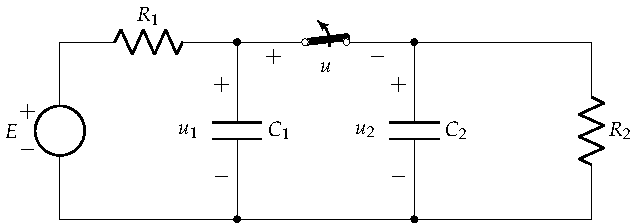
\includegraphics{figuras/BT4_02.pdf}
\end{center}

\subsection*{Solución}

\begin{enumerate}
    \item El circuito para $t<0$ tiene el interruptor cerrado. Al estar alimentado por CC, los condensadores se comportan como circuitos abiertos, por lo que:
    \begin{align*}
        &I=\dfrac{E}{R_{eq}}=\dfrac{15}{200+100}=0.05\,\si{\ampere}\\
        &U_{R100}=R_{100}\cdot I=100\cdot 0.05=5\,\si{\volt}\\
        &u_{C1}(0^-)=u_{C2}(0^-)=U_{R100}=5\,\si{\volt}
    \end{align*}
    Por continuidad, se deduce que $u_{C1}(0^-)=u_{C1}(0^+)=u_{C2}(0^-)=u_{C2}(0^+)=5\,\si{\volt}$
    \item Para $t>0$, el interruptor se abre, quedando dos circuitos independientes. 
    \begin{enumerate}
        \item \textbf{Circuito de la izquierda}\\
        La resistencia de Thévenin vista desde los extremos del condensador, cuando se anula la fuente de tensión, es:
    \begin{equation*}
        R_{th1}=200\,\Omega
    \end{equation*}
    siendo la constante de tiempo:
    \begin{equation*}
        \tau_1=R_{th1}\;C_1=200\cdot 2\cdot10^{-6}=0.0004\,\si{\second}
    \end{equation*}
    Para la respuesta en régimen permanente, se sustituye de nuevo el condensador por un circuito abierto (por estar alimentado en CC), siendo entonces:
    \begin{equation*}
        u_{\infty1}(t)=E=15\,\si{\volt}
    \end{equation*}
    \item \textbf{Circuito de la derecha}\\
        La resistencia de Thévenin vista desde los extremos del condensador es:
    \begin{equation*}
        R_{th2}=100\,\Omega
    \end{equation*}
    siendo la constante de tiempo:
    \begin{equation*}
        \tau_2=R_{th2}\;C_2=100\cdot 4\cdot10^{-6}=0.0004\,\si{\second}
    \end{equation*}
    Para la respuesta en régimen permanente, al no haber ninguna fuente de alimentación:
    \begin{equation*}
        u_{\infty2}(t)=0\,\si{\volt}
    \end{equation*}
    \end{enumerate}
    \item Las expresiones completas de $u_1(t)$ y $u_2(t)$ son:
    \begin{align*}
        u_1(t)&=\left(5-15 \right)\,\mathrm{e}^{-2500\,t}+15=15-10\,\mathrm{e}^{-2500\,t}\,\si{\volt}\\
        u_2(t)&=\left(5-0 \right)\,\mathrm{e}^{-2500\,t}+0=5\,\mathrm{e}^{-2500\,t}\,\si{\volt}
    \end{align*}
\end{enumerate}


\section{Enunciado}
El interruptor del circuito de la figura lleva cerrado un timepo
  que se considera infinito. En el instante $t=0$, se abre y permanece
  en dicha posición definitivamente. Hállese la expresión de $u(t)$ e
  $i(t)$ para $t>0$.

  Datos:\; $E = \qty{36}{\volt}$;\; $R_1 = \qty{2}{\ohm}$;\;
  $R_2 = \qty{4}{\ohm}$; $R_3 = \qty{3}{\ohm}$;\;
  $C = \qty{3}{\milli\farad}$; $L = \qty{6}{\milli\henry}$

\begin{center}
  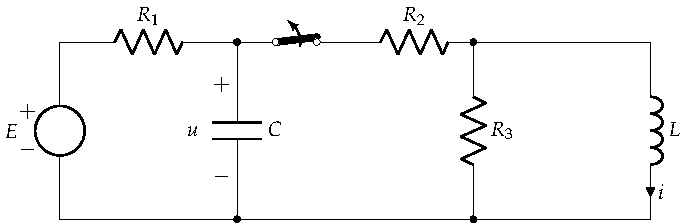
\includegraphics{figuras/BT4_03.pdf}
\end{center}

\subsection*{Solución}

\begin{enumerate}
    \item El circuito para $t<0$ tiene el interruptor cerrado. Al estar alimentado por CC, el condensador se comporta como circuito abierto y la bobina como cortocircuito, por lo que la resistencia de $3\Omega$ queda cortocircuitada:
    \begin{align*}
        &I=\dfrac{E}{R_{eq}}=\dfrac{36}{2+4}=6\,\si{\ampere}\\
        &i(0^-)=I=6\,\si{\ampere}\\
        &u(0^-)=E-I\,R_2=36-6\cdot 2=24\,\si{\volt}
    \end{align*}
    Por continuidad, se deduce que $i(0^-)=i(0^+)=6$ A y $u(0^-)=u(0^+)=24\,\si{\volt}$
    \item Para $t>0$, el interruptor se abre, quedando dos circuitos independientes. 
    \begin{enumerate}
        \item \textbf{Circuito de la izquierda}\\
        La resistencia de Thévenin vista desde los extremos del condensador, cuando se anula la fuente de tensión, es:
    \begin{equation*}
        R_{th1}=2\,\Omega
    \end{equation*}
    siendo la constante de tiempo:
    \begin{equation*}
        \tau_1=R_{th1}\;C=2\cdot 3\cdot10^{-3}=0.006\,\si{\second}
    \end{equation*}
    Para la respuesta en régimen permanente, se sustituye de nuevo el condensador por un circuito abierto (por estar alimentado en CC), siendo entonces:
    \begin{equation*}
        u_{\infty}(t)=E=36\,\si{\volt}
    \end{equation*}
    \item \textbf{Circuito de la derecha}\\
        La resistencia de Thévenin vista desde los extremos de la bobina es:
    \begin{equation*}
        R_{th2}=3\,\Omega
    \end{equation*}
    siendo la constante de tiempo:
    \begin{equation*}
        \tau_2=\dfrac{L}{R_{th2}}=\dfrac{6\cdot 10^{-3}}{3}=0.002\,\si{\second}
    \end{equation*}
    Para la respuesta en régimen permanente, al no haber ninguna fuente de alimentación:
    \begin{equation*}
        i_{\infty}(t)=0\,\si{\ampere}
    \end{equation*}
    \end{enumerate}
    \item Las expresiones completas de $u(t)$ e $i(t)$ son:
    \begin{align*}
        u(t)&=\left(24-36 \right)\,\mathrm{e}^{-166.67\,t}+36=36-12\,\mathrm{e}^{-166.67\,t}\,\si{\volt}\\
        i(t)&=\left(6-0 \right)\,\mathrm{e}^{-500\,t}+0=6\,\mathrm{e}^{-500\,t}\,\si{\ampere}
    \end{align*}
\end{enumerate}


\section{Enunciado}
El circuito de la figura lleva en esa posición un tiempo que se
  puede considerar infinito. En el instante $t=0$, ambos interruptores
  cambian su posición. Calcular la expresión de $u(t)$ para $t>0$.

  Datos:\; $E_1 = \qty{40}{\volt}$;\; $R_1 = \qty{20}{\ohm}$;\;
  $R_2 = \qty{60}{\ohm}$;\; $R_3 = \qty{3}{\ohm}$;\;
  $R_4 = \qty{6}{\ohm}$;\; $C = \qty{0.5}{\milli\farad}$;\;
  $e_2(t) = 120 \, \cos(1000t)\unit{\volt}$

\begin{center}
  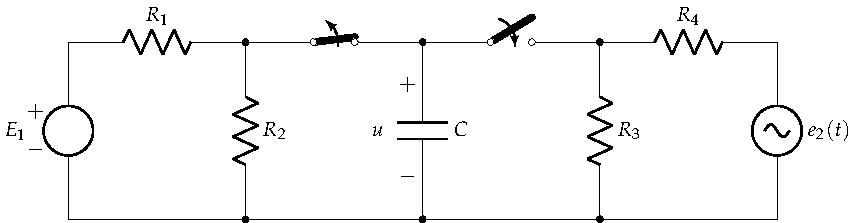
\includegraphics{figuras/BT4_04.pdf}
\end{center}

\subsection*{Solución}

\begin{enumerate}
    \item El circuito para $t<0$ tiene el interruptor de la izquierda cerrado y el de la derecha abierto. Por tanto, el condensador está alimentado por CC, comportándose como un circuito abierto:
    \begin{align*}
        &I=\dfrac{E_{CC}}{R_{eq}}=\dfrac{40}{20+60}=0.5\,\si{\ampere}\\
        &U_{R60}=I\,R_{60}=0.5\cdot 60=30\,\si{\volt}\\
        &u(0^-)=U_{R60}=30\,\si{\volt}
    \end{align*}
    Por continuidad, se deduce que $u(0^-)=u(0^+)=30\,\si{\volt}$ 
    \item Para $t>0$, el interruptor de la izquierda se abre y se cierra el de la derecha, quedando el condensador alimentado por la fuente de CA. 
    La resistencia de Thévenin vista desde los extremos del condensador, cuando se anula la fuente de tensión, es:
    \begin{equation*}
        R_{th}=\dfrac{6\cdot 3}{6+3}=2\,\Omega
    \end{equation*}
    siendo la constante de tiempo:
    \begin{equation*}
        \tau=R_{th}\cdot C=2\cdot0.5\cdot10^{-3}=0.001\,\si{\second}
    \end{equation*}
    Para la respuesta en régimen permanente, se trabaja con fasores (considerando el valor eficaz), teniendo un circuito formado por dos resistencias (6 y 3 $\Omega$) y un condensador ($\overline{X}_C=\frac{1}{\mathrm{j}\,\omega\,C}=\frac{1}{\mathrm{j}\,1000\cdot 0.5\cdot 10^{-3}}=-\mathrm{j}\,2\,\Omega$). La tensión del condensador:
    \begin{align*}
        &\overline{Z}_{eq}=6+\dfrac{3\,(-\mathrm{j}2)}{3\,-\mathrm{j}2}=7.06\phase{-11.31^\circ}\,\Omega\\
        &\overline{I}_T=\dfrac{\overline{E}_{CA}}{\overline{Z}_{eq}}=\dfrac{\frac{120}{\sqrt{2}}\phase{0^\circ}}{7.06\phase{-11.31^\circ}}=12.02\phase{11.31^\circ} \,\si{\ampere}\\
        &\overline{U}_{\textrm{paralelo}}=\overline{U}_C=\overline{I}_T\cdot\overline{Z}_{\textrm{paralelo}}=12.02\phase{11.31^\circ}\cdot \dfrac{3\,(-\mathrm{j}2)}{3\,-\mathrm{j}2}=20\phase{-45^\circ}\,\si{\volt}\\
        &u_\infty(t)=20\sqrt{2}\,\cos\left(1000\,t-\frac{\pi}{4}\right)\,\si{\volt} \quad\rightarrow\quad u_\infty(0^+)=20\,\si{\volt}
    \end{align*}
    \item La expresión completa de $u(t)$ es:
    \begin{equation*}
        u(t)=\left(30-20 \right)\,\mathrm{e}^{-1000\,t}+20\sqrt{2}\,\cos\left(1000\,t-\frac{\pi}{4}\right)=10\,\mathrm{e}^{-1000\,t}+20\sqrt{2}\,\cos\left(1000\,t-\frac{\pi}{4}\right)\,\si{\volt}
    \end{equation*}
\end{enumerate}


\section{Enunciado}
En el circuito de la figura se abre el interruptor después de un
  tiempo suficientemente grande para considerar que el circuito
  funcionaba en régimen permanente. Expresar las formas de onda de
  $i_1$, $i_2$ y $u_L$ para $t>0$.

  Datos:\; $e(t)=220\sqrt{2}\,\cos(100\pi\,t)\,\unit{\volt}$;\;
  $L = \qty{0.2}{\henry}$;\; $R_1 = \qty{25}{\ohm}$;\;
  $R_2 = \qty{275}{\ohm}$
  
\begin{center}
  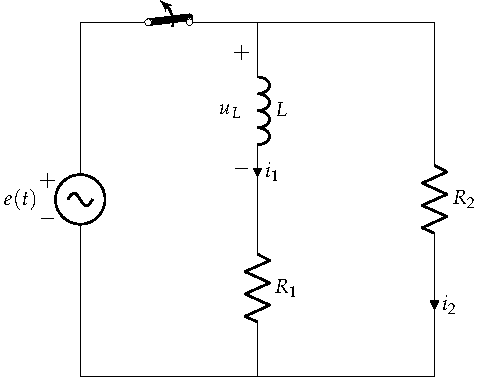
\includegraphics{figuras/BT4_05.pdf}
\end{center}

\subsection*{Solución}


\begin{enumerate}
    \item El circuito para $t<0$ tiene el interruptor cerrado:
    \begin{align*}
        &\overline{X}_L=\mathrm{j}\,\omega\,L=\mathrm{j}\,2\cdot\pi\cdot 50\cdot 0.2=\mathrm{j}\,20\pi\,\Omega\\
        &\overline{I}_1=\dfrac{\overline{E}}{R_{25}+\overline{X}_L}=\dfrac{220\phase{0}}{25+\mathrm{j}\,20\pi}=3.25\phase{-68.303^\circ}\,A \quad\rightarrow\quad i_1(t)=3.25\sqrt{2}\,\cos(100\pi\,t-1.192)\,\si{\ampere}
    \end{align*}
    Por tanto, en $t=0^-$ la corriente en la bobina es $i_1(0^-)=1.7\,\si{\volt}=i_1(0^+)$, por continuidad.
    \item Para $t>0$, el interruptor se abre, quedando el circuito sin alimentación externa. La resistencia de Thévenin vista desde los extremos de la bobina es:
    \begin{equation*}
        R_{th}=275+25=300\,\Omega
    \end{equation*}
    siendo la constante de tiempo:
    \begin{equation*}
        \tau=\dfrac{L}{R_{th}}=\dfrac{0.2}{300}=0.00067\,\si{\second}
    \end{equation*}
    Para la respuesta en régimen permanente, al no haber fuente de alimentación:
    \begin{equation*}
        i_{\infty1}=0
    \end{equation*}
    \item La expresión completa de $i_1(t)$ es:
    \begin{equation*}
        i_1(t)=\left(1.7-0 \right)\,\mathrm{e}^{-1500\,t}+0=1.7\,\mathrm{e}^{-1500\,t}\,\si{\ampere}
    \end{equation*}
\end{enumerate}
La tensión en la bobina se puede determinar a partir de su relación con la corriente:
\begin{align*}
    &u_L(t)=L\,\diff{\,i(t)}{t}\\
    &\diff{\,i(t)}{t}=1.7\cdot (-1500)\,\mathrm{e}^{-1500\,t}=-2550\,\mathrm{e}^{-1500\,t}\,\si{\ampere\per\second}\\
    & u_L(t)=L\,\diff{\,i(t)}{t}=0.2\cdot (-2550)\,\mathrm{e}^{-1500\,t}=-510\,\mathrm{e}^{-1500\,t}\,\si{\volt}
\end{align*}
y, al estar únicamente la malla de resistencias y bobina:
\begin{equation*}
    i_2(t)=-1.7\,\mathrm{e}^{-1500\,t}\,\si{\ampere}
\end{equation*}


\section{Enunciado}
En el circuito de la figura, en $t = 0$ se cierra el
  interruptor. Obtener la expresión analítica de la intensidad $i(t)$,
  para $t > 0$.

  Datos:\; $E = \qty{10}{\volt}$;\; $L = \qty{0.2}{\henry}$;\;
  $I_g = \qty{1}{\ampere}$;\; $R_1 = \qty{10}{\ohm}$;\;
  $\alpha = \qty{3}{\ohm}$

\begin{center}
  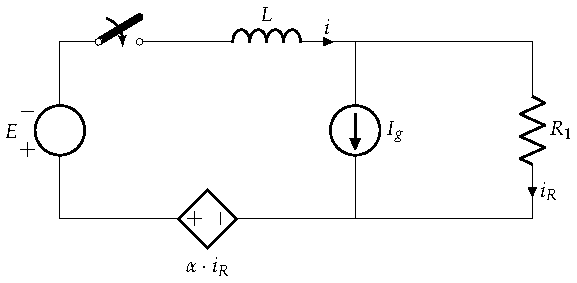
\includegraphics{figuras/BT4_06.pdf}
\end{center}

\subsection*{Solución}

\begin{enumerate}
    \item El circuito para $t<0$ tiene el interruptor abierto, por lo que:
    \begin{align*}
        i(0^-)=0\,\si{\ampere}
    \end{align*}
    Por continuidad, $i(0^-)=i(0^+)=0\,\si{\ampere}$ 
    \item Para $t>0$, el interruptor se cierra. Para calcular la resistencia de Thévenin apagamos los generadores independientes y conectamos un generador de prueba en los terminales de la bobina. Obtenemos:
    \begin{align*}
      \epsilon_0 &= 3\cdot i_r + 10 \, I_0\\
      i_r &= - I_0\\
      R_{th} &= \frac{\epsilon_0}{I_0} = \qty{7}{\ohm}
    \end{align*}
    siendo la constante de tiempo:
    \begin{equation*}
        \tau=\dfrac{L}{R_{th}}=\dfrac{0.2}{7}=0.0286\,\si{\second}
    \end{equation*}
    Para la respuesta en régimen permanente, la bobina sería un cortocircuito (por ser CC), por lo que:
    \begin{align*}
      -10 + 3 \cdot i_r &= 10 \cdot i_r \quad\rightarrow\quad i_r = -\frac{10}{7}\,\unit{\ampere}\\
      i_{\infty} &= I_g + i_r = -\frac{3}{7}\,\unit{\ampere}
    \end{align*}
    
    \item La expresión completa de $i(t)$ es:
    \begin{equation*}
        i(t)=\left(0-\left(-\dfrac{3}{7}\right) \right)\,\mathrm{e}^{-35\,t}+\left(-\dfrac{3}{7}\right)=\dfrac{3}{7}\,(\mathrm{e}^{-35\,t}-1)\;\si{\ampere}
    \end{equation*}
\end{enumerate}



\section{Enunciado}

El interruptor de la figura ha estado cerrado por un tiempo prolongado y en $t = 0$ se abre.

\begin{minipage}{0.5\linewidth}
  \center{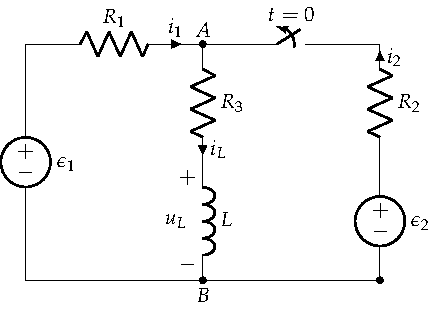
\includegraphics{figuras/BT4_CondicionesIniciales_bobina.pdf}}
\end{minipage}
\begin{minipage}{0.5\linewidth}
  \hspace{20mm} Datos:
  \begin{align*}
    R_1 &= \SI{5}{\ohm}\\
    R_2 &= \SI{5}{\ohm}\\
    R_3 &= \SI{2}{\ohm}\\
    L &= \SI{3.5}{\milli\henry}\\
    \epsilon_1 &= \SI{24}{\volt}\\
    \epsilon_2 &= \SI{12}{\volt}
  \end{align*}
\end{minipage}

\medskip

Con esta información, se debe calcular:
\begin{enumerate}
\item Valores de $i_1(0^+)$, $i_2(0^+)$, $i_L(0^+)$, $u_L(0^+)$ y
  $u_{AB}(0^+)$.
\item Expresión de $i_L(t)$ para $t > 0$.
\item Expresiones de $u_L(t)$ y $u_{AB}(t)$ para $t > 0$.
\end{enumerate}

\subsection*{Solución}

En el circuito en $t <0$, la bobina se comporta como un
cortocircuito. Resolviendo por mallas el circuito resultante, obtenemos
los valores para $t = 0^-$:

\vspace{-4mm}
\begin{align*}
  i_L(0^-) &= \qty{4}{\ampere}\\
  i_1(0^-) &= \qty{3.2}{\ampere}\\
  i_2(0^-) &= \qty{0.8}{\ampere}
\end{align*}

En la bobina podemos plantear la condición de continuidad,
$i_L(0^-) = i_L(0^+)$, que nos permite obtener los valores para
$t = 0^+$, una vez abierto el interruptor:

\vspace{-4mm}
\begin{align*}
  i_L(0^+) &= \qty{4}{\ampere}\\
  i_1(0^+) &= i_L(0^+)\\
  i_2(0^+) &= \qty{0}{\ampere}\\
  u_L(0^+) &= \epsilon_1 - i_1(0^+) \cdot R_1 - i_L(0^+) \cdot R_3 = -\qty{4}{\volt}\\
  u_{AB}(0^+) &= \epsilon_1 - i_1(0^+) \cdot R_1 = \qty{4}{\volt}
\end{align*}

Analizamos ahora el circuito para $t > 0$, en el que el interruptor
está abierto. La resistencia vista por la bobina es
$R_{th} = R_1 + R_3 = \qty{7}{\ohm}$. Por tanto:

\begin{equation*}
  \tau = \frac{L}{R_{th}} = \qty{500}{\micro\second}
\end{equation*}

Obtenemos la respuesta forzada analizando el circuito en régimen
permanente, en el que la bobina se comportará como un cortocircuito:

\begin{equation*}
  i_{L,\infty}(t) = \frac{\epsilon_1}{R_1 + R_3} = \qty{3.43}{\ampere}
\end{equation*}

\vspace{2mm}
Obtenemos la respuesta natural apagando la fuente $\epsilon_1$. La ec. diferencial correspondiente a este circuito es:

\[
  (R_1 + R_3) \cdot i_{L,n}(t) \,+\, L \; \diff{\,i_{L,n}(t)}{t} \, = \,  0
\]

\vspace{2mm}
Cuya solución es de la forma:

\begin{equation*}
  i_{L,n}(t) = K \cdot e^{-t/\tau} = K \cdot e^{-2000 \cdot t}
\end{equation*}

\vspace{2mm}
Para obtener la constante $K$, recurrimos a la condición inicial
$i_L(0^+) = \qty{4}{\ampere}$:

\begin{equation*}
  K = i_L(0^+) - i_{L,\infty}(0^+) = 4 - 3.43 = \qty{0.57}{\ampere}
\end{equation*}

Por tanto:

\begin{equation*}
  i_L(t) = i_{L,n}(t) + i_{L,\infty}(t) = 3.43 + 0.57 \cdot e^{-2000 \cdot t} \;\unit{\ampere}
\end{equation*}

\vspace{2mm}
Con este resultado podemos obtener las tensiones en el circuito:

\begin{equation*}
  u_L(t) = L \cdot \diff{\, i_L}{t} = 3.5\cdot 10^{-3} \cdot 0.57 \cdot 2\cdot 10^{3} \cdot e^{-2000 \cdot t} = - 4 \cdot e^{-2000 \cdot t} \;\unit{\volt}
\end{equation*}

\begin{equation*}
  u_{AB}(t) =  u_L(t) + R_3 \cdot i_L(t) = 6.86 - 2.86 \cdot e^{-2000 \cdot t} \;\unit{\volt}
\end{equation*}

\vspace{2mm}
Comprobamos que estas expresiones concuerdan con los resultados
obtenidos para $u_L(0^+)$ y $u_{AB}(0^+)$.

\section{Enunciado}

El interruptor del circuito de la figura lleva abierto un tiempo
indefinido. En el instante $t= 0$ se cierra este interruptor. Hay que
obtener:
\begin{enumerate}
\item Valores de las tensiones $u_1(0^+)$, $u_2(0^+)$, $u_3(0^+)$ y
  $u_c(0^+)$.
\item Expresión temporal de la tensión $u_c(t)$ para $t > 0$.
\item Expresiones temporales de $u_2(t)$ y $u_3(t)$ para $t > 0$.
\end{enumerate}

\begin{minipage}{0.5\linewidth}
  \center{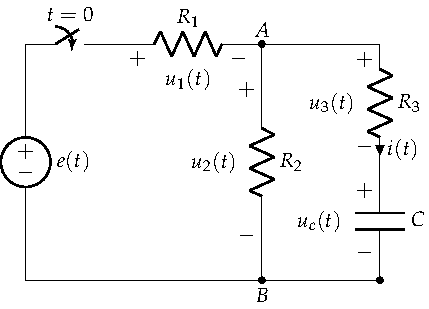
\includegraphics{figuras/BT4_CondicionesIniciales_condensador.pdf}}
\end{minipage}
\begin{minipage}{0.5\linewidth}
  \hspace{20mm} Datos:
    \begin{align*}
    e(t) &= 10\,\unit{\volt}\\
    R_1 &= R_2 = 2 \,\unit{\ohm}\\
    R_3 &= 4 \,\unit{\ohm}\\
    C &= 1 \,\unit{\farad}
  \end{align*}
\end{minipage}

\subsection*{Solución}

\begin{enumerate}
\item

  En $t < 0$, dado que el interruptor lleva abierto un tiempo largo, la fuente
  está aislada del circuito, por lo que el condensador se comporta como un circuito
  abierto.

  \vspace{3mm}
  En estas condiciones
  $u_c(0^-) = \qty{0}{\volt}$. Debido a la condición de
  continuidad, $u_c(0^+) = u_c(0^-) = \qty{0}{\volt}$.

\begin{minipage}{0.4\linewidth}
  Con este resultado podemos determinar el resto de tensiones del
  circuito en $t = 0^+$, teniendo en cuenta que el
  interruptor está cerrado y el condensador es equivalente a un
  cortocircuito ($u_c(0^+) = \qty{0}{\volt}$).
\end{minipage}
\hfill
\begin{minipage}{0.55\linewidth}
  \center{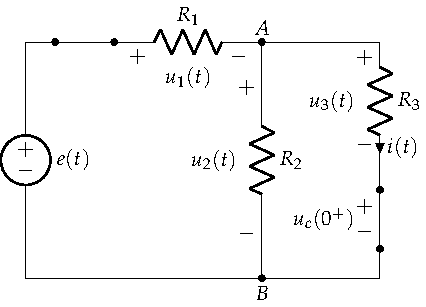
\includegraphics{figuras/BT4_CondicionesIniciales_condensador0+.pdf}}
\end{minipage}

En este circuito, $R_2$ y $R_3$ están en paralelo entre sí, siendo
$R_{23} = \frac{R_2 \cdot R_3}{R_2 + R_3}$. Esta resistencia paralelo
está en serie con $R_1$, formando un divisor de tensión. Por tanto:
\begin{align*}
  u_2(0^+) = u_3(0^+) &= e(t) \cdot \frac{R_{23}}{R_1 + R_{23}} = \qty{4}{\volt}\\
  \textrm{Por 2LK:}\qquad u_1(0^+) &= e(t) - u_2(0^+) = \qty{6}{\volt}
\end{align*}

\item

  Analizamos ahora el circuito para $t > 0$, obteniendo la respuesta forzada y la respuesta natural:


  \begin{minipage}{0.5\linewidth}
    Planteamos el equivalente de Thévenin (apagando la fuente de tensión) para calcular la resistencia vista por el condensador:

  \[
    R_{th} = R_3 + \frac{R_1 \cdot R_2}{R_1 + R_2} = \qty{5}{\ohm}
  \]

  Por tanto:
  \begin{equation*}
    \tau = \frac{C}{G_{th}} = \qty{5}{\second}
  \end{equation*}
\end{minipage}
\begin{minipage}{0.5\linewidth}
  \center{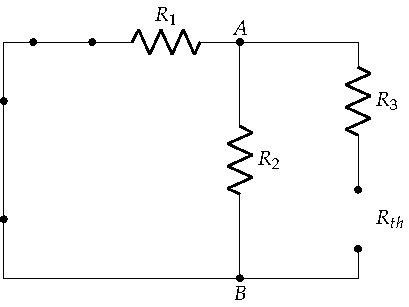
\includegraphics{figuras/BT4_CondicionesIniciales_condensador_Rth.pdf}}
\end{minipage}

Obtenemos la respuesta forzada analizando el circuito en régimen
permanente, en el que el condensador se comportará como un circuito
abierto:

\begin{equation*}
  u_{C,\infty}(t) = e(t) \cdot \frac{R_2}{R_1 + R_2} = \qty{5}{\volt}
\end{equation*}

Obtenemos la respuesta natural resolviendo la ec. homogénea (apagando la fuente $e(t)$). Su solución es:
\begin{equation*}
  u_{C,n}(t) = A \cdot e^{-t/\tau} = A \cdot e^{-0.2\, t}
\end{equation*}

Para obtener la constante $A$, recurrimos a la condición inicial
$u_C(0^+) = \qty{0}{\volt}$:

\begin{equation*}
  A = u_{C,n}(t=0^+) = u_C(0^+) - u_{C,\infty}(0^+) = 0 - 5 = \qty{-5}{\volt}
\end{equation*}

Por tanto:
\begin{equation*}
  u_C(t) = u_{C,n}(t) + u_{C,\infty}(t) = 5 \cdot (1 - e^{-0.2\, t}) \;\unit{\volt}
\end{equation*}

\vspace{2mm}
\item Con este resultado podemos obtener la corriente que circula por
  el condensador:

\begin{equation*}
  i_C(t) = C \cdot \diff{\,u_C}{t} = (-5)\cdot(-0.2)\cdot e^{-0.2\, t} = e^{-0.2\, t} \,\unit{\ampere}
\end{equation*}

y a partir de esta, las tensiones en las resistencias:
\begin{align*}
  u_{R3}(t) &=  R_3 \cdot i_C(t) = 4 \cdot e^{-0.2\, t} \;\unit{\volt}\\[3pt]
  u_{R2}(t) &=  u_{R3}(t) + u_C(t) = 5 - e^{-0.2\, t} \;\unit{\volt}
\end{align*}
    
  
\end{enumerate}

\section{Enunciado}

Calcular la corriente $i(t)$ para $t > 0$.

\begin{minipage}{0.5\textwidth}
  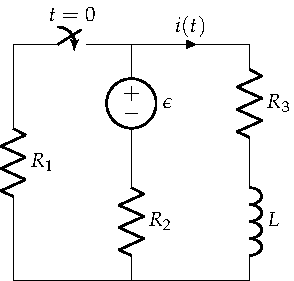
\includegraphics{figuras/FM_4_2}
\end{minipage}
\hfill
\begin{minipage}{0.5\textwidth}
  Datos:
  \begin{align*}
    \epsilon &= \SI{24}{\volt}\\
    R_1 &= \SI{8}{\ohm}\\
    R_2 &= \SI{4}{\ohm}\\
    R_3 &= \SI{4}{\ohm}\\
    L &= \SI{15}{\henry}
  \end{align*}
\end{minipage}

\subsection*{Solución}

Calculamos las condiciones iniciales ($t = 0^-$). Dibujamos el circuito para $t < 0$ y obtenemos:

\vspace{4mm}
\begin{minipage}{0.5\textwidth}
  \centering{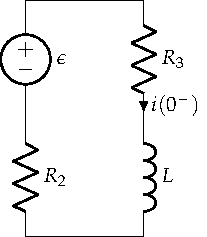
\includegraphics{figuras/FM_4_2_t0-}}
\end{minipage}
\begin{minipage}{0.2\textwidth}
  \begin{equation*}
    i(t) = \frac{\epsilon}{R_2 + R_3}
  \end{equation*}
\end{minipage}

\vspace{4mm}
Por tanto, $i(0^-) = \SI{3}{\ampere}$. Al tratarse de una bobina,
$i(0^+) = i(0^-) = \SI{3}{\ampere}$.

\vspace{2mm}
A continuación dibujamos el circuito para $t > 0$ para obtener la
respuesta natural y la respuesta forzada.

\vspace{2mm}
Para obtener la respuesta natural, apagamos las fuentes. En este
circuito obtenemos:

\vspace{2mm}
\begin{minipage}{0.5\textwidth}
  \centering 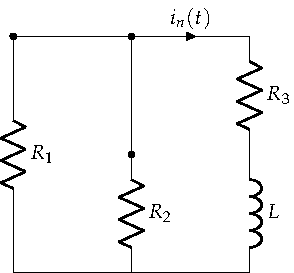
\includegraphics{figuras/FM_4_2_natural}
\end{minipage}
\begin{minipage}{0.4\textwidth}
  \begin{align*}
    R_{th} &= R_3 + (R_1 \parallel R_2) = \frac{20}{3}\,\si{\ohm}\\[3pt]
    \tau &= \frac{L}{R_{th}} = \frac{9}{4}\,\si{\second}\\[3pt]
    i_n(t) &= A \cdot e^{-\frac{t}{\tau}} = A \cdot e^{-4t/9}
  \end{align*}
\end{minipage}

\vspace{4mm}
Queda por determinar la constante de integración.

\vspace{3mm}
Para obtener la respuesta forzada volvemos a activar las fuentes. En
este circuito obtenemos:

\vspace{2mm}
\begin{minipage}{0.5\textwidth}
  \centering 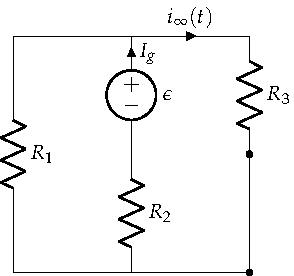
\includegraphics{figuras/FM_4_2_forzada}
\end{minipage}
\begin{minipage}{0.4\textwidth}
  \begin{align*}
    I_g &= \frac{\epsilon}{R_2 + (R_1 \parallel R_3)}\\[3pt]
    i_\infty(t) &= I_g \cdot \frac{G_3}{G_3 + G_1} = \SI{2.4}{\ampere}
  \end{align*}
\end{minipage}

\vspace{4mm}
Con estos dos resultados podemos obtener la respuesta completa:
\begin{align*}
  i(t) &= i_n(t) + i_\infty(t)\\[3pt]
  i(t) &= A \cdot e^{-4t/9} + 2.4 \;\si{\ampere}
\end{align*}

Para determinar la constante de integración recurrimos a las
condiciones iniciales:
\begin{align*}
  i(0^+) &= A + 2.4 \\
  i(0^+) &= 3 \\
  A &= 0.6
\end{align*}

Por tanto:
\begin{equation*}
  i(t) = 0.6 \cdot e^{-4t/9} + 2.4 \,\si{\ampere}
\end{equation*}

\section{Enunciado}

Calcular la tensión en bornes del condensador para $t > 0$.

\vspace{3mm}
\begin{minipage}{0.5\textwidth}
  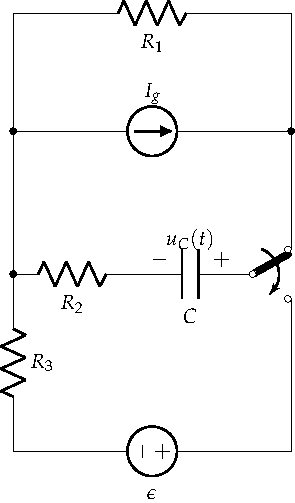
\includegraphics[scale=0.85]{figuras/FM_4_3}
\end{minipage}
\hfill
\begin{minipage}{0.5\textwidth}
  Datos:
  \begin{align*}
    \epsilon &= \SI{20}{\volt}\\
    I_g &= \SI{4}{\ampere}\\
    R_1 &= \SI{6}{\ohm}\\
    R_2 &= \SI{4}{\ohm}\\
    R_3 &= \SI{12}{\ohm}\\
    C &= \SI[parse-numbers=false]{1/16}{\farad}      
  \end{align*}

\end{minipage}

\subsection*{Solución}

Calculamos las condiciones iniciales ($t = 0^-$). Dibujamos el circuito para $t < 0$ y obtenemos:

\vspace{3mm}
\begin{minipage}{0.3\textwidth}
  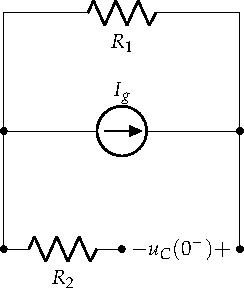
\includegraphics{figuras/FM_4_3_t0-}
\end{minipage}
\begin{minipage}{0.7\textwidth}
  \begin{equation*}
    u_C(t) = I_g \cdot R_1 
  \end{equation*}
\end{minipage}

\vspace{2mm}
Por tanto, $u_c(0^-) = \SI{24}{\volt}$. Al tratarse de un condensador,
$u_C(0^+) = u_C(0^-) = \SI{24}{\volt}$.

\vspace{3mm}
A continuación dibujamos el circuito para $t > 0$ para obtener la
respuesta natural y la respuesta forzada.

\vspace{3mm}
Para obtener la respuesta natural apagamos las fuentes. En este
circuito obtenemos:

\vspace{2mm}
\begin{minipage}{0.3\textwidth}
  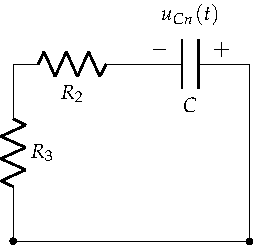
\includegraphics{figuras/FM_4_3_natural}
\end{minipage}
\begin{minipage}{0.7\textwidth}
  \begin{align*}
    R_{th} &= R_2 + R_3 = \SI{16}{\ohm}\\
    \tau &= C/G_{th} = \SI{1}{\second}\\
    u_{Cn}(t) &= A \cdot e^{-\frac{t}{\tau}} = A \cdot e^{-t}
  \end{align*}
\end{minipage}

\vspace{4mm}
Queda por determinar la constante de integración.

\vspace{3mm}
Para obtener la respuesta forzada, volvemos a activar las fuentes. En
este circuito obtenemos:

\begin{minipage}{0.3\textwidth}
  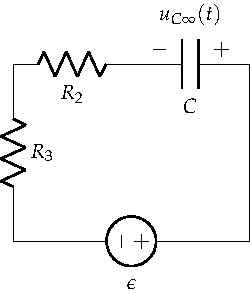
\includegraphics{figuras/FM_4_3_forzada}
\end{minipage}
\begin{minipage}{0.7\textwidth}
  \begin{equation*}
    u_{c\infty}(t) = \epsilon = \SI{20}{\volt}
  \end{equation*}
\end{minipage}

\vspace{3mm}
Con estos dos resultados podemos obtener la respuesta completa:
\begin{align*}
  u_C(t) &= u_{Cn}(t) + u_{c\infty}(t)\\
  u_C(t) &= A \cdot e^{-t} + 20
\end{align*}

\vspace{2mm}
Para determinar la constante de integración recurrimos a las
condiciones iniciales:
\begin{align*}
  u_C(0^+) &= A + 20\\
  u_C(0^+) &= 24\\
  A &= \SI{4}{\volt}
\end{align*}

Por tanto:
\begin{equation*}
  u_C(t) = 4 \cdot e^{-t} + 20 \;\si{\volt}
\end{equation*}

\section{Enunciado}

Determina las corrientes $i_L(t)$ e $i_1(t)$ para $t > 0$.

\begin{minipage}{0.7\textwidth}
  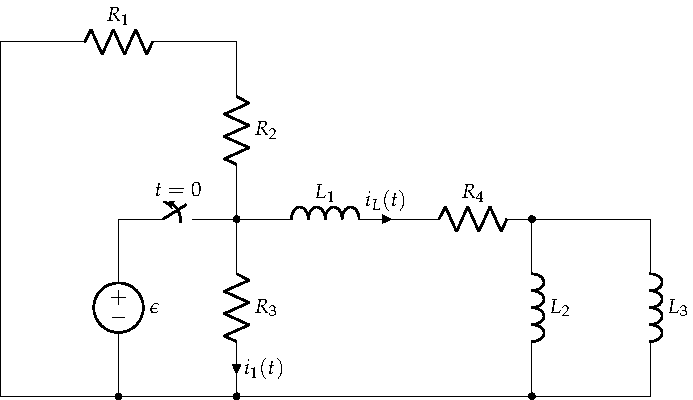
\includegraphics{figuras/HKD84}
\end{minipage}
\hfill
\begin{minipage}{0.3\textwidth}
  Datos:
  \begin{align*}
    \epsilon &= \SI{18}{\volt}\\
    R_1 &= \SI{120}{\ohm}\\
    R_2 &= \SI{60}{\ohm}\\
    R_3 &= \SI{90}{\ohm}\\
    R_4 &= \SI{50}{\ohm}\\
    L_1 &= \SI{1}{\milli\henry}\\
    L_2 &= \SI{2}{\milli\henry}\\
    L_3 &= \SI{3}{\milli\henry}
  \end{align*}
\end{minipage}

\subsection*{Solución}

Calculamos las condiciones iniciales ($t = 0^-$). 
Dibujamos el circuito para $t < 0$:

\begin{center}
  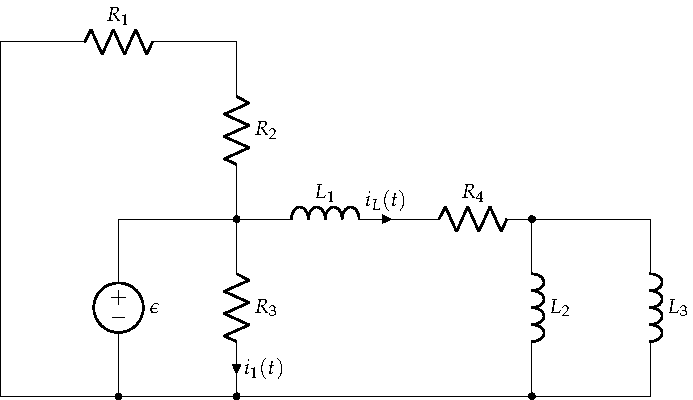
\includegraphics[scale=0.9]{figuras/HKD84_t0-}
\end{center}

\vspace{2mm}
Obtenemos:
\begin{equation*}
  i_L(t) = \frac{\epsilon}{R_4} = \SI{360}{\milli\ampere}
\end{equation*}

\vspace{3mm}
Al tratarse de una bobina,
$i_L(0^+) = i_L(0^-) = \SI{360}{\milli\ampere}$.

\vspace{3mm}
En este circuito podemos calcular
$i_1(0^-) = \frac{\epsilon}{R_3} = \SI{200}{\milli\ampere}$. Este
valor nos servirá de referencia cuando calculemos $i_1(t)$.

\vspace{3mm}
A continuación dibujamos el circuito para $t > 0$ para obtener la
respuesta natural y la respuesta forzada. En el circuito resultante no
hay fuentes, por lo que únicamente tendremos respuesta natural.

\begin{center}
  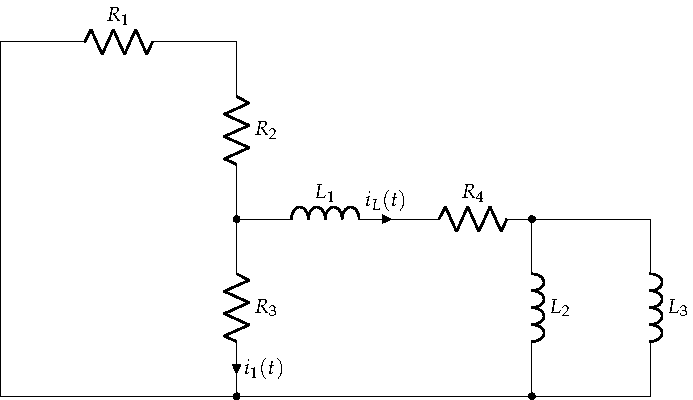
\includegraphics[scale=0.9]{figuras/HKD84_natural}
\end{center}

\vspace{-2mm}
  \begin{align*}
    L_{eq} &= L_1 + L_2||L_3 = \SI{2.2}{\milli\henry}\\
    R_{th} &= (R_1 + R_2) || R_3 + R_4  = \SI{110}{\ohm}\\
    \tau &= L_{eq}/R_{th} = \SI{20}{\micro\second}\\
    i_{Ln}(t) &= A \cdot e^{-\frac{t}{\tau}} = A \cdot e^{-5 \cdot 10^{4} \cdot t}
  \end{align*}

  Queda por determinar la constante de integración. Dado que la
  respuesta forzada es 0 podemos calcular directamente esta constante
  con la respuesta natural y las condiciones iniciales:
\begin{align*}
  i_L(t) &= i_{Ln}(t) = A \cdot e^{-5 \cdot 10^{4} \cdot t}\\
  i_L(0^+) &= A = 0.36
\end{align*}

Por tanto:
\begin{equation*}
  i_L(t) = 0.36 \cdot e^{-5 \cdot 10^{4} \cdot t}\;\si{\ampere}
\end{equation*}

\vspace{2mm}
Para calcular la corriente $i_1(t)$ usamos un divisor de corriente a
partir de $i_L(t)$:
\begin{equation*}
  i_1(t) = -i_L(t) \cdot \frac{1/R_3}{1/R_3 + 1/(R_1 + R_2)} = -0.24 \cdot e^{-5 \cdot 10^{4} \cdot t}\;\si{\ampere}
\end{equation*}

\vspace{3mm}
En el primer apartado habíamos obtenido
$i_1(0^-) = \SI{200}{\milli\ampere}$. Con esta ecuación obtenemos
$i_1(0^+) = -\SI{240}{\milli\ampere}$. Los valores no coinciden porque
en una resistencia no hay condición de continuidad.

\section{Enunciado}

El circuito de la figura ha alcanzado el régimen permanente con el
interruptor cerrado. El interruptor se abre en $t = 0$. Calcula las
expresiones de la tensión en bornes del condensador y de la corriente
por la bobina para $t > 0$.

\vspace{4mm}

\begin{minipage}{0.6\textwidth}
  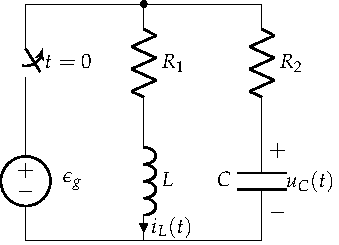
\includegraphics[scale=1]{figuras/FM_4_8}
\end{minipage}
\hfill
\begin{minipage}{0.4\textwidth}
  Datos:
  \begin{align*}
    \epsilon_g &= \SI{10}{\volt}\\
    R_1 &= \SI{10}{\ohm}\\
    R_2 &= \SI{5}{\ohm}\\
    L &= \SI{2.5}{\henry}\\
    C &= \SI{0.2}{\farad}      
  \end{align*}
\end{minipage}

\subsection*{Solución}

Calculamos las condiciones iniciales ($t = 0^-$). Dibujamos el circuito para $t < 0$ y obtenemos:

\vspace{3mm}
\begin{minipage}{0.3\textwidth}
  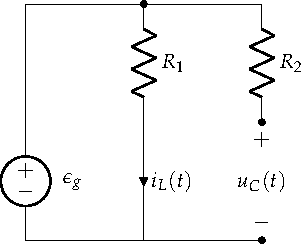
\includegraphics{figuras/FM_4_8_t0-}
\end{minipage}
\begin{minipage}{0.7\textwidth}
  \begin{align*}
    u_C(t) &= \SI{10}{\volt}\\
    i_L(t) &= \frac{\epsilon_g}{R_1} = \SI{1}{\ampere}
  \end{align*}
\end{minipage}

\vspace{4mm}
Por tanto, $u_C(0^+) = u_C(0^-) = \SI{10}{\volt}$ \;y\;
$i_L(0^+) = i_L(0^-) = \SI{1}{\ampere}$.

\vspace{3mm}
A continuación dibujamos el circuito para $t > 0$ para obtener la
respuesta natural y la respuesta forzada. En el circuito resultante no
hay fuentes, por lo que no habrá respuesta forzada.

\vspace{3mm}
\begin{minipage}{0.3\textwidth}
  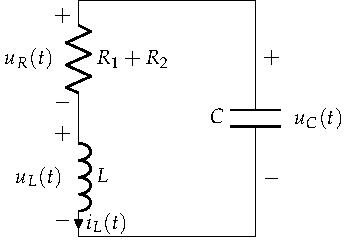
\includegraphics{figuras/FM_4_8_natural}
\end{minipage}
\begin{minipage}{0.7\textwidth}
  \begin{align*}
    \alpha &= \frac{R}{2L} = \SI{3}{\second}^{-1}\\
    \omega_0 &= \frac{1}{\sqrt{LC}} = \sqrt{2}\,\si{\radian\per\second}
  \end{align*}
\end{minipage}

\vspace{3mm}
Dado que $\alpha > \omega_0$, se trata de un transitorio
sobreamortiguado:

\begin{align*}
  s_1 &= -\alpha + \sqrt{\alpha^2 - \omega_0^2} = \SI{-0.354}{\second}^{-1}\\
  s_2 &= -\alpha - \sqrt{\alpha^2 - \omega_0^2} = \SI{-5.645}{\second}^{-1}\\
  i_L(t) &= A_1 \cdot e^{-0.354 \cdot t} + A_2 \cdot e^{-5.645 \cdot t}
\end{align*}

\vspace{3mm}
Para determinar las constantes de integración recurrimos a las
condiciones iniciales:

\vspace{3mm}
\begin{minipage}{0.3\textwidth}
  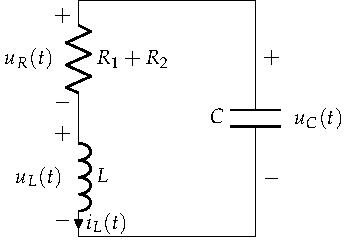
\includegraphics[scale=1]{figuras/FM_4_8_natural}
\end{minipage}
\begin{minipage}{0.7\textwidth}
  \begin{align*}
    u_R(t) + u_L(t) &= u_C(t)\\
    u_L(0^+) &= u_C(0^+) - u_R(0^+)\\
    u_R(0^+) &= (R_1 + R_2) \cdot i_L(0^+) = \SI{15}{\volt}\\
    u_L(0^+) &= 10 - 15 = \SI{-5}{\volt}
  \end{align*}
\end{minipage}

\vspace{5mm}
Por tanto:
\begin{align*}
  i_L(0^+) &= \SI{1}{\ampere}\\[3pt]
  \diff{i_L(t)}{t}[t = 0^+] &= \frac{1}{L} \cdot u_L(0^+) = \SI{-2}{\ampere\per\second}
\end{align*}

\vspace{2mm}
Con estos resultados, particularizamos la ecuación de $i_L(t)$ para
$t = 0$ y así planteamos las ecuaciones para obtener $A_1$ y $A_2$:
\begin{align*}
  i_L(0^+) &= A_1 + A_2 = 1\\[3pt]
  \diff{\, i_L(t)}{t}[t = 0^+] &= A_1 \cdot s_1 + A_2 \cdot s_2 = -2
\end{align*}

Por tanto:
\begin{align*}
  A_1 &= \qty{0.689}{\ampere}\\
  A_2 &= \qty{0.311}{\ampere}
\end{align*}

Finalmente:
\begin{equation*}
  i_L(t) = 0.689 \cdot e^{-0.354 \cdot t} + 0.311 \cdot e^{-5.645 \cdot t}\;\si{\ampere}\\
\end{equation*}

\vspace{3mm}
Para obtener la tensión en el condensador recurrimos a la LKV:
\begin{align*}
  u_C(t) &= u_R(t) + u_L(t) = \\
         &= (R_1 + R_2) \cdot i_L(t) + L \; \diff{\, i_L(t)}{t} = \\
         &= 9.728 \cdot e^{-0.354 \cdot t} + 0.275 \cdot e^{-5.645 \cdot t} \;\si{\volt}
\end{align*}

\section{Enunciado}
En el circuito de la figura, calcular la tensión $u_C(t)$ para $t > 0$.

\begin{minipage}{0.5\linewidth}
  \begin{center}
    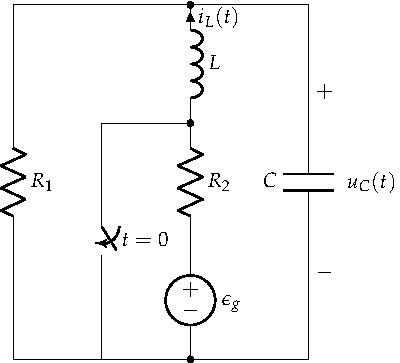
\includegraphics{figuras/FM_4_9.pdf}
  \end{center}
\end{minipage}
\begin{minipage}{0.5\linewidth}
  \center{Datos:}
  \begin{align*}
    \epsilon_g &= \SI{4}{\volt}\\
    R_1 &= \SI{2}{\ohm}\\
    R_2 &= \SI{2}{\ohm}\\
    L &= \SI{1}{\henry}\\
    C &= \SI{0.25}{\farad}      
  \end{align*}
\end{minipage}

\subsection*{Solución}

Calculamos las condiciones iniciales ($t = 0^-$). Dibujamos el
circuito para $t < 0$ y obtenemos:

\vspace{3mm}
\begin{minipage}{0.3\textwidth}
  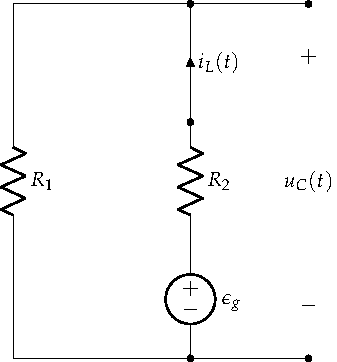
\includegraphics[scale=0.9]{figuras/FM_4_9_t0-}
\end{minipage}
\begin{minipage}{0.7\textwidth}
  \begin{align*}
    i_L(t) &= \frac{\epsilon_g}{R_1 + R_2} = \SI{1}{\ampere}\\[10pt]
    u_C(t) &= R_1 \cdot i_L(t) = \SI{2}{\volt}    
  \end{align*}
\end{minipage}

\vspace{3mm}
Por tanto, $u_C(0^+) = u_C(0^-) = \SI{2}{\volt}$ \; y
\;
$i_L(0^+) = i_L(0^-) = \SI{1}{\ampere}$.

\vspace{3mm}
A continuación dibujamos el circuito para $t > 0$, para obtener la
respuesta natural y la respuesta forzada. En el circuito resultante no
hay fuentes, por lo que no habrá respuesta forzada.

\vspace{3mm}
\begin{minipage}{0.3\textwidth}
  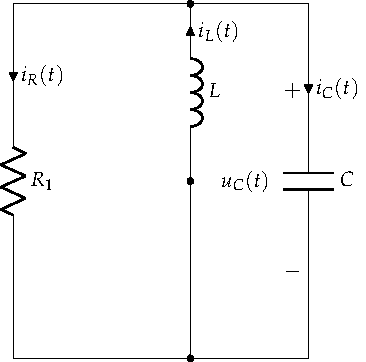
\includegraphics[scale=0.9]{figuras/FM_4_9_natural}
\end{minipage}
\begin{minipage}{0.7\textwidth}
  \begin{align*}
    \alpha &= \frac{G}{2C} = \SI{1}{\second}^{-1}\\
    \omega_0 &= \frac{1}{\sqrt{LC}} = 2\si{\radian\per\second}
  \end{align*}
\end{minipage}

\bigskip

Dado que $\alpha < \omega_0$, se trata de un transitorio
subamortiguado:
\begin{align*}
  \omega_d &= \sqrt{\omega_0^2 - \alpha^2} = \sqrt{3}\;\si{\radian\per\second}\\
  u_C(t) &= [B_1 \cdot \cos(\sqrt{3} \cdot t) + B_2 \cdot \sin(\sqrt{3} \cdot t)] \cdot e^{-t}
\end{align*}

\vspace{2mm}
Para determinar las constantes de integración recurrimos a las
condiciones iniciales:

\vspace{3mm}
\begin{minipage}{0.3\textwidth}
  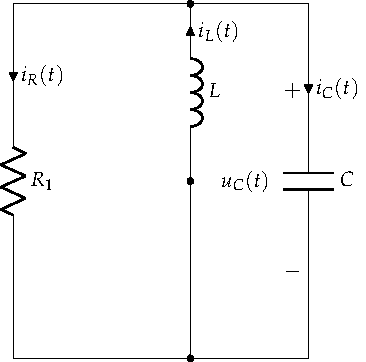
\includegraphics[scale=0.9]{figuras/FM_4_9_natural}
\end{minipage}
\begin{minipage}{0.7\textwidth}
  \begin{align*}
    i_C(0^+) &= i_L(0^+) - i_R(0^+)\\
    i_R(0^+) &= G_1 \cdot u_C(0^+) = \SI{1}{\ampere}\\
    i_C(0^+) &= 1 - 1 = \SI{0}{\ampere}
  \end{align*}
\end{minipage}

\vspace{5mm}
Por tanto:
\begin{align*}
  u_C(0^+) &= \SI{2}{\volt}\\[3pt]
  \diff{u_C(t)}{t}[t = 0^+] &= \frac{1}{C} \cdot i_C(0^+) = \SI{0}{\volt\per\second}
\end{align*}

Con estos resultados, particularizamos la ecuación de $u_C(t)$ para
$t = 0$ y así planteamos las ecuaciones para obtener $B_1$ y $B_2$:
\begin{align*}
  u_C(0^+) &= B_1 = \SI{2}{\volt}\\[3pt]
  \diff{u_C(t)}{t}[t = 0^+] &= \Big[-e^{-t} \cdot (2\cos(\sqrt{3}t) + B_2\sin(\sqrt{3}t)) +\\
           & \qquad + e^{-t} \cdot (-2\sqrt{3}\sin(\sqrt{3}t) + \sqrt{3} B_2\cos(\sqrt{3}t)) \Big]_{t = 0^+}=\\
           &= 0
\end{align*}

Por tanto:
\begin{align*}
  B_1 &= 2\\
  B_2 &= \frac{2\sqrt{3}}{3}
\end{align*}

Finalmente:
\begin{equation*}
u_C(t)= \mathrm{e}^{-t}\left[2\,\cos(\sqrt{3}\,t)+\dfrac{2}{\sqrt{3}}\,\sin(\sqrt{3}\,t)\right]=\dfrac{4\sqrt{3}}{3}\,\mathrm{e}^{-t}\,\sin\left(\sqrt{3}\,t+\dfrac{\pi}{6}\right) \;\si{\volt}
\end{equation*}


\section{Enunciado}
En el circuito de la figura el interruptor ha estado cerrado durante un tiempo elevado, y en $t = 0$ se abre. En estas condiciones se debe determinar:

\begin{enumerate}
\item Tipo de transitorio presente en el circuito.

\item Condiciones iniciales de las siguientes variables del circuito: $u_C(0^+)$, $i_L(0^+)$, $i_C(0^+)$, $u_L(0^+)$.
\item Valores en régimen permanente de las siguientes variables del circuito: $u_C(\infty)$, $i_L(\infty)$, $i_C(\infty)$, $u_L(\infty)$.
\item Expresión de la corriente $i_L(t)$ para  $t > 0$.
\item Expresión de la tensión $u_C(t)$ para  $t > 0$.
\end{enumerate}

\begin{minipage}{0.3\linewidth}
  Datos:


  \begin{align*}
    E_g &= \SI{500}{\volt}\\   
    R_{1} &= \SI{375}{\ohm}\\ 
    R_{2} &=\SI{125}{\ohm}\\ 
    L_1 &= \SI{40}{\milli\henry}\\ 
    C &= \SI{1}{\micro\farad}
  \end{align*}
\end{minipage}
\begin{minipage}{0.7\linewidth}
  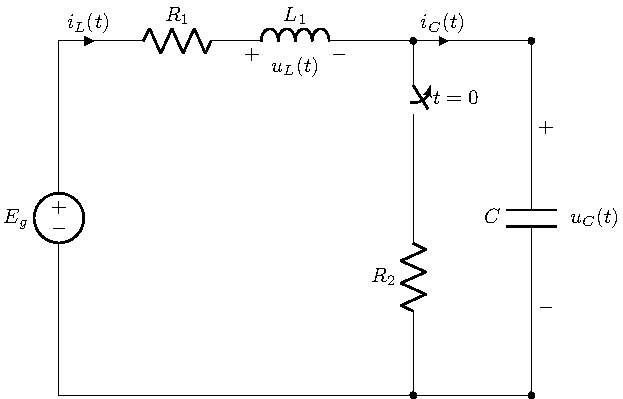
\includegraphics{figuras/E1_RLC.pdf}
\end{minipage}

\subsection*{Solución}

\begin{enumerate}

\item Tipo de transitorio

La siguiente figura representa el circuito para $t > 0$.

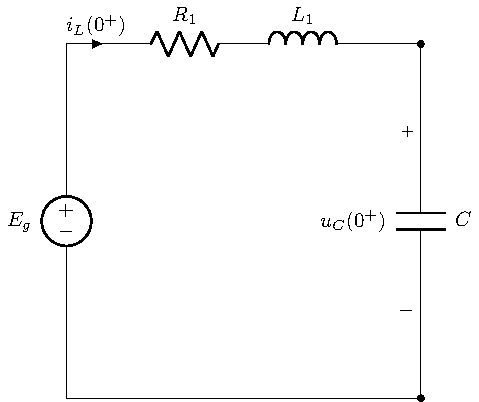
\includegraphics{figuras/E1_RLC_0+.pdf}

Al apagar las fuentes en este circuito comprobamos que se trata de un RLC serie. Por tanto podemos calcular:
\begin{align*}
  \alpha &= \frac{R_1}{2L_1} = \SI{4687.5}{\second}^{-1}\\[3pt]
  \omega_0 &= \frac{1}{\sqrt{L_1C}} = \SI{5000}{\radian\per\second}\\[3pt]
  \xi &= \frac{\alpha}{\omega_0} = 0.9375\\[3pt]
  \omega_d &= \sqrt{\omega_0^2 - \alpha^2} = \SI{1740}{\radian\per\second}
\end{align*}

\vspace{1mm}
Dado que $\alpha < \omega_0$ ($\xi < 1$), el transitorio es subamortiguado.

\vspace{2mm}

\item Condiciones iniciales

  La siguiente figura representa el circuito para $t < 0$ en régimen permanente, con las variables particularizadas para $t = 0^-$.

  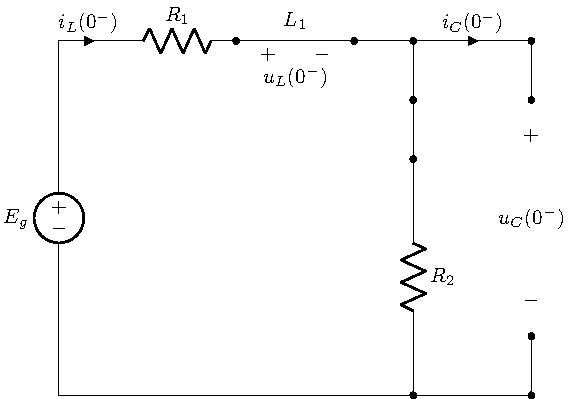
\includegraphics{figuras/E1_RLC_0-.pdf}

\vspace{3mm}
  En este circuito, teniendo en cuenta las condiciones de continuidad, se puede deducir que:
  \begin{align*}
    i_L(0^+) = i_L(0^-) &= \SI{1}{\ampere}\\
    u_C(0^+) = u_C(0^-) &= \SI{125}{\volt}
  \end{align*}

  Además, considerando el circuito en $t=0^+$:
  \[
    E_g = u_R(0^+) + u_L(0^+) + u_C(0^+)
  \]

  Por tanto:
  \[
    u_L(0^+) = E_g - R_1 \cdot i_L(0^+) - u_C(0^+) = \SI{0}{\volt} 
  \]

    \vspace{2mm}
  Finalmente, $\quad i_C(0^+) = i_L(0^+) = \SI{1}{\ampere}$.
  
  \vspace{2mm}

\item Valores en régimen permanente.

  El circuito en régimen permanente está abierto debido al condensador. Por tanto:
  \begin{align*}
    u_c(\infty) & = \SI{500}{\volt}\\
    u_L(\infty) & = \SI{0}{\volt}\\
    i_c(\infty) & = \SI{0}{\ampere}\\
    i_L(\infty) & = \SI{0}{\ampere}
  \end{align*}

    
\item Expresión de $i_L(t)$

  La expresión genérica de la corriente es:
  \[
    i_L(t) = i_L(\infty) + e^{-\alpha t} \left(A_1 \sen(\omega_d t) + A_2 \cos(\omega_d t)\right)
  \]

  siendo $\omega_d = \sqrt{\omega_o^2 - \alpha^2} = \SI{1740}{\radian\per\second}$.

  \vspace{3mm}
  Teniendo en cuenta las condiciones iniciales y el valor en régimen permanente obtenemos:
  \begin{align*}
    i_L(0^+) = 1 &= A_2\\
    \diff{\, i_L(t)}{t}[t = 0^+] = \frac{1}{L} \; u_L(0^+) = 0 &= -\alpha A_2 + A_1 \omega_d
  \end{align*}

  La solución de este sistema es:
  \begin{align*}
    A_1 &= \frac{\alpha}{\omega_d} = \qty{2.7}\ampere\\
    A_2 &= \qty{1}{\ampere}\\
  \end{align*}
  
  Por tanto:
  \begin{align*}
        i_L(t) &= e^{-\alpha \cdot t} \left(\frac{\alpha}{\omega_d} \sen(\omega_d t) + \cos(\omega_d t)\right)\\
    i_L(t) &= e^{-4687.5 \cdot t} \left(2.7 \sen(1740\cdot t) + \cos(1740 \cdot t)\right)\\
               &= 2.88 \cdot e^{-4687.5 \cdot t} \cdot \sen(1740\cdot t + 0.3547) \;\si{\ampere}
  \end{align*}

\vspace{2mm}

\item Expresión de $u_C(t)$

  A partir de la expresión anterior podemos calcular la correspondiente a la tensión en el condensador, teniendo en cuenta que:
  \begin{align*}
    u_C(t) &= E_g - R_1 \cdot i_L(t) - L_1 \; \diff{\; i_L(t)}{t} \\[10pt]
    u_C(t) &= 500 - e^{-4687.5 \cdot t} \left[435.9 \sen(1740\cdot t) + 375 \cos(1740 \cdot t)\right]\\[5pt]
           &= 500 - 575.01 \cdot e^{-4687.5 \cdot t} \cdot  \sen(1740\cdot t + 0.7104)\;\si{\volt}
  \end{align*}

  Este resultado se puede comprobar mediante las condiciones iniciales:
    \begin{align*}
    u_C(0^+) &= \qty{125}{\volt}\\[4pt]
    \diff{\, u_C(t)}{t}[t = 0^+] &= \frac{1}{C} \; i_C(0^+) = 10^6\,\si{\volt\per\second}\\
  \end{align*}

\end{enumerate}

%%% Local Variables:
%%% mode: latex
%%% TeX-master: "Problemas_TC"
%%% ispell-local-dictionary: "castellano"
%%% End:


